\chapter{Backend}
        Il backend è stato sviluppato in Python \cite{Python} usando il framework Flask \cite{Flask}.\\
        \'E stato scelto Python perchè è un linguaggio già usato internamente per lo sviluppo di plugin e tool interni.

        \section{Specifica e documentazione}
            Prima della fase di sviluppo è stata predisposto un periodo di design dell' API.\\
            Questo processo ha prodotto un file di specifica (descritta nel paragrafo 
            \ref{openapi}).\\\\
            Questa fase preliminare allo sviluppo è durata circa una settimana ed è servita per 
            individuare difficoltà tecniche in modo preliminare che sono sate discusse con il team.\\
            In questo modo \'e stato risparmiato tempo durante lo sviluppo, evitando di dover ristrutturare l'applicazione successivamente.\\
            Questa specifica come vedremo in seguito è servita anche a produrre automaticamente una pagina di documentazione (\ref{apidoc}).
            
            \subsection{Specifica in linguaggio OpenAPI\label{openapi}}
                La Specifica dell'API è stata scritta in formato OpenAPI \cite{OpenAPI}.\\
                Questo file può essere scritto in linguaggio JSON o YML, io ho scelto il secondo perchè
                sintatticamente più leggero e usa l'indentazione per separare le sezioni, facilitandone dunque la scrittura. \\
                Questo formato ci consente di descrivere tutte le chiamate che il server 
                mette a disposizione, specificando:
                \begin{itemize}
                    \item Il formato dell'URI 
                    \item Il metodo
                    \item Il formato di interscampio dei dati (json, xml ecc) 
                    \item La struttura della risposta
                    \item Come deve essere strutturata la richiesta perch\'e essa sia valida
                    \item I codici di errori e la loro semantica specifica nel contesto dell'applicazione
                \end{itemize}
                
            \subsection{Documentazione\label{apidoc}}
                Inoltre da questa specifica è possibile generare la documentazione, in pagina statica html,
                tramite l'utilizzo di diverse CLI\footnote{\textbf{Command Line Interface} - Interfaccia a linea di comando}.\\
                Io ho scelto ReDoc, perchè mette a disposizione diverse vendore-extension, cioè sezioni che
                se specificate provedono una maggiore customizzazione della pagina generata.\\
                Queste estensioni sono state usate per sezioni di codice di esempio riguardo a come effettuare una chiamata al server, e per aggiungere riferimenti a file markdown esterni da includere nella documentazione.\\
                
                \begin{figure}[h]
                    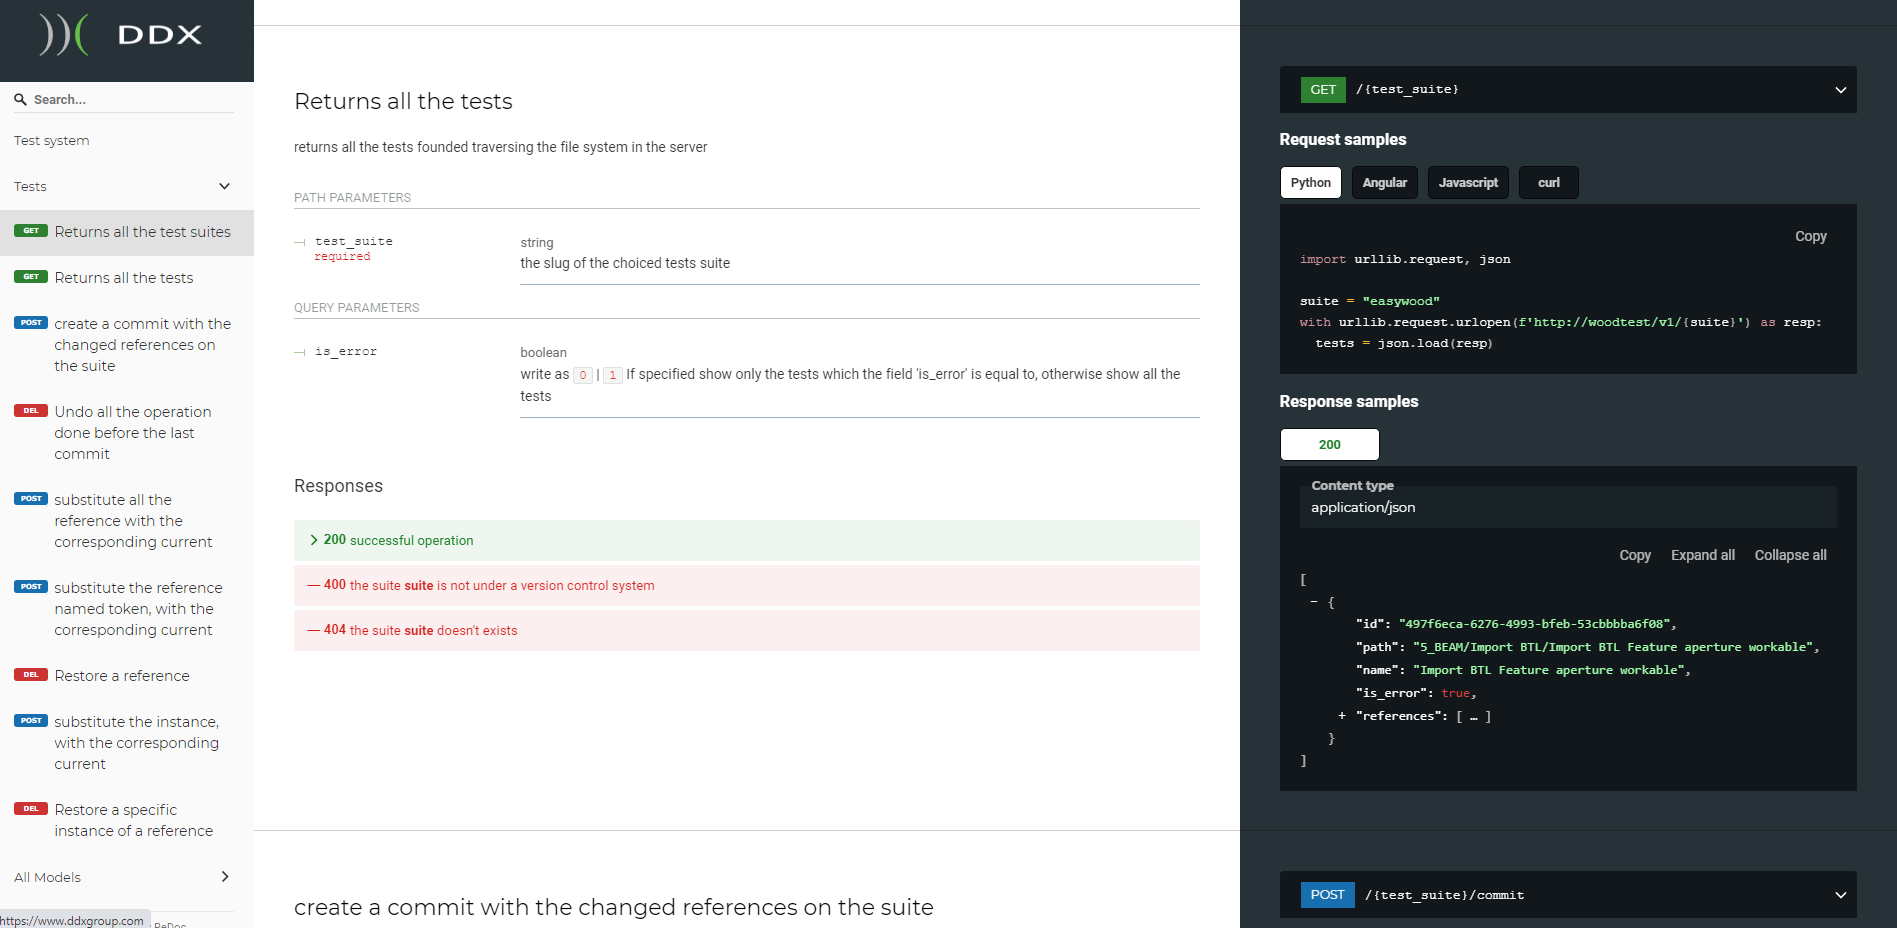
\includegraphics[width=\textwidth]{images/documentation.png}
                    \caption{Uno screenshot della pagina di documentazione generata dal processo di CI}
                \end{figure}

            \subsection{Continous integration}
                Il processo di scrittura della documentazione è stato aggiunto a una pipeline di CI
                \footnote{\textbf{Continous Integration} - L'integrazione continua consiste nell'integrare gli ambienti di sviluppo dei diversi sviluppatori tramite processi di build, testing ecc... eseguiti da un server condiviso}.
                Questo processo si occupa, solo se il file .yml di specifica viene modificato, di 
                rigenerare il file html di documentazione.\\
                Questo file viene successivamente servito in modo da rendere la documentazione 
                disponibile online e sempre aggiornata con le specifiche.

    \section{Tecnologie Utilizzate}  
        \subsection{Python}
            Python \'e un linguaggio di scripting, interpretato ad alto livello, ovvero la gestione della memoria viene effettuata da un sistema di garbage collection e non delegata allo sviluppatore.\\
            Questo linguaggio è stato scelto siccome \'e usato per lo scripting all'interno di altri applicativi esistenti e dunque gi\'a familiare a molti sviluppatori.\\
            
            Tra le varie librerie prodotte \'e presente anche un modulo per lanciare i test e inviare i risultati agli sviluppatori via e-mail.\\
            Questo modulo non è stato utilizzato all'interno del test report ma l'uso dello stesso linguaggio ha contribuito a mantenere la code-base pi\'u uniforme.
        \subsection{Flask}  
            Flask \'e un \textit{micro}Framework per la creazione di servizi web, esso consente di creare applicazioni complete o API (come nel nostro caso).\\
            La sua peculiarit\'a \'e la minimalit\'a e consente si scrivere applicazioni in modo rapido riducendo al minimo la parte di codice che si occupa della gestione dell'interfaccia HTTP \cite{HTTP}.\\
            Questo \'e possibile grazie agli strumenti di introsprezione del codice offerti dal linguaggio come i decoratori.\\

            Esso \'e stato scelto perch\'e l'applicazione, essendo destinata all'uso interno, non necessitava di gestioni di rete di basso livello per coordinare grandi quantit\'a di richieste.\\
            L'attenzione principale \'e stata invece posta sulla riusabilità dell'API.

    \section{Interazione con i sistemi di controllo di versione}           
        Un sistema di controllo di versione è un software distribuito che si occupa di tenere traccia di tutti i cambiamenti effettuati su un progetto.\\
        Lo sviluppatore dopo ogni modifica si occuperà di registrarla nel sistema, creando quello che viene definito un commit.\\
        Questi software consentono di ripristinare versioni precedenti e avere uno storico dei cambiamenti effettuati.\\
        Le tests suite sono revisionate con un sistema di versioning.\\
        
        L'API oltre alla modifica, aggiunta o rimozione dei test si occupa anche di versionare queste azioni nel sistema usato dalla suite.\\
        Per sapere quali sono le modifiche alla suite effettuate, il servizio si avvale di \textit{staging area}. \\
        Sono aree intermedie salvate in locale che consentono di formattare e rivedere le modifiche prima di creare il commit.\\
        La creazione del commit avviene tramite un endpoint specifico. \\

        Internamente vengono usati sia Git \cite{Git} che SubVersion (SVN) \cite{SubVersion} e una specifica del report è supportare entrambi in modo trasparente allo sviluppatore.\\
        Questa funzionalità nasce da una necessità futura di effettuare una migrazione delle test suite revisionate attualmente con Svn a Git.\\
            
    \section{Struttura dell'API}
        Nel processo di design dell'API si è scelto di adottare i principi architetturali REST \cite{REST}.\\
        Il primo punto di questa filosofia consiste nel poter assegnare un indirizzo (detto \textit{URI} ovvero \textit{Unique Resource Identifier}) a ogni risorsa dell'applicazione.\\
        L'URI deve essere univoco e descrittivo riguardo al tipo di risorsa che si sta richiedendo.\\
        
        La comunicazione si basa sul protocollo HTTP e coinvolge due tipi di attori chiamati client e server.\\
        Il server si occupa di esporre l'API e i client di effettuare una serie di richieste per manipolare le risorse a seconda delle loro necessità.\\
        Ogni messaggio scambiato tra i client e il server si occupa di effettuare una singola operazione su un oggetto.\\
        La richiesta è composta da un metodo che descrive quale azione compiere, e un URI che indica il soggetto.\\
        
        Ogni URI \'e composto da diverse sezioni, tra esse il \textit{path} che definisce una collocazione logica della risorsa all'interno dell'applicazione.\\
        Gli indirizzi delle risorse sono creati ragruppando quelli che hanno informazioni associate.\\
        Per esempio se si vuole accedere a un test viene identificata prima la suite di appartenenza e poi l'id del test: \verb|/easywood/doh2hw527jm|.\\
        Per riferirsi alle reference invece ci si riferisce al test di appartenenza e successivamente viene specificata la distribuzione, in questo modo: \verb|/easywood/doh2hw527jm/64bit|.\\
        
        I metodi principali sono:
        
        \begin{itemize}
            \item \textbf{GET} Per ottenere le informazioni relative a una risorsa
            \item \textbf{POST} Per la creazione di nuove risorse
            \item \textbf{PUT} Si riferisce alla modifica di elementi già presenti nel sistema
            \item \textbf{DELETE} Per eliminare dati
        \end{itemize}
        
        Ogni API definisce una semantica specifica per le sue operazioni.\\
        Nel nostro caso non ogni metodo è stato definito dal servizio, perché altre operazioni come la creazione di un test o una suite esulano dalle responsabilità dell'applicazione.\\
        
        Per i test è disponibile il metodo GET per ottenerne il nome, il path relativo e le sue reference.\\
        Ognuna di esse è composta da stato di errore e di stato di registrazione nel sistema (registrato, modificato o non registrato).\\
        Per le reference sono disponibili anche i metodi PUT e DELETE. PUT è per definizione da specifica di REST idempotente e si occupa della modifica di una risorsa, percio nel nostro caso registra nel sistema le eventuali modifiche/differenze ottenute durante la sessione di test, se la reference si trova in stato di errore essa verrà sostituita dal suo file current, altrimenti se non è in errore o è già stata modificata non verrà effettuata alcuna operazione.\\
        
        I soggetti dell'API sono le operazioni di registrazione dei test, perciò l'operazione di DELETE assume la semantica di "undo", ovvero ripristino dello stato del sistema all'ultima configurazione registrata nel controllo di versione.\\
        
        Il server risponderà con un pacchetto HTTP composto da uno status code e un corpo contente il risultato dell'operazione.\\
        Lo status code è un codice di 3 cifre che descrive se l'operazione è andata a buon fine o il tipo di errore (per esempio: risorsa non trovata, utente non autorizzato ecc...).\\
        